\documentclass[border=3mm]{standalone}
\usepackage{amsmath}
\usepackage{tikz}
\usepackage{pgfplots}
\pgfplotsset{compat=1.18}
\begin{document}
	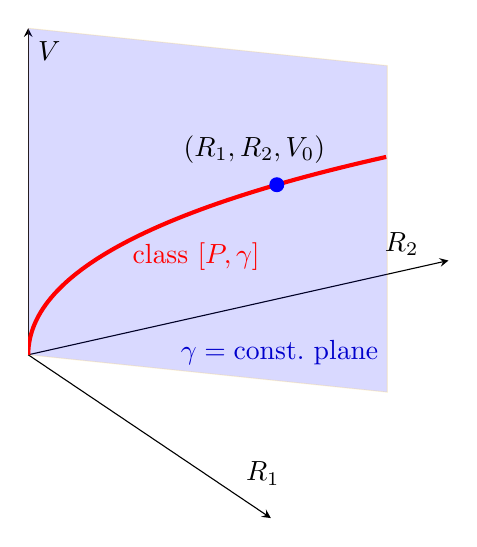
\begin{tikzpicture}
		\begin{axis}[
			width=10cm, height=9cm,
			view={60}{30}, % Ángulo de perspectiva tridimensional
			xlabel={$R_1$},
			ylabel={$R_2$},
			zlabel={$V$}, % El voltaje en el eje vertical (Z)
			xmin=0, xmax=12,
			ymin=0, ymax=12,
			zmin=0, zmax=5,
			axis lines=center,
			grid=both,
			ticks=none, % Gráfico puramente conceptual
			enlargelimits=false
			]

			% 1. Plano vertical de atenuación constante (R_1 = R_2)
			% Usamos mesh/rows para estructurar la superficie correctamente en PGFPlots
			\addplot3[
			surf,
			domain=0:6.5,
			domain y=0:5,
			samples=2,
			samples y=2,
			opacity=0.15,
			fill=blue,
			faceted color=none] (x, x, y); % (R_1 = x, R_2 = x, V = y)
			\addplot3[
			domain=0:3.6,
			samples=60,
			samples y=0,
			line width=1.5pt,red] ({0.5*x^2}, {0.5*x^2}, x); % (r_1, r_2, V)
			% Etiquetas flotantes informativas
			\node[color=blue!80!black, anchor=south west] at (axis cs:3.6,2,0.2)
			{$\gamma = \text{const.}$ plane};
			\node[color=red, anchor=south east] at (axis cs:5,4,1.7)
			{class $[P, \gamma]$};
			% 3. Punto específico fijando un Voltaje V_0 = 3
			% Si V_0 = 3, entonces R_1 = R_2 = 0.5 * 3^2 = 4.5
			\addplot3[only marks, mark=*, mark size=2.5pt, color=blue]
			    coordinates {(4.5, 4.5, 3.0)};
			\node[anchor=west] at (axis cs:2, 3, 3.2)
			   {$(R_1, R_2, V_0)$};

		\end{axis}
	\end{tikzpicture}
\end{document}
